\documentclass[12pt]{article}
\usepackage[italian]{babel}
\usepackage{graphicx}
\usepackage[section]{placeins}
\usepackage{amsmath}% http://ctan.org/pkg/amsmath
\usepackage{enumitem}
\usepackage{graphicx}
\usepackage[section]{placeins}

\title{Business Intelligence e Servizi per la Finanza}
\author{Giuseppe Facchi}
\date{A.A. 2020-2021}

\begin{document}
\maketitle
\newpage
\tableofcontents
\newpage

\section{Introduzione alla Finanza}
Gli strumenti sono chiamati \textbf{securities}
\paragraph{Security} Un qualsiasi strumento finanziario con un valore finanziario utilizzabile e negoziabile. Tiplogie:
\begin{itemize}
    \item \textbf{Debito}: Security risk-free (Bonds, depositi ecc.)
    \item \textbf{Equity}: Azioni delle compagnie
    \item \textbf{Derivatives}: Il loro valore dipende da altre variabili (\textbf{futures}, \textbf{forward}, swaps, \textbf{options})
\end{itemize}
Si trovano nei \textbf{mercati finanziari}
\subsection{Bonds}
I \textbf{bond} sono considerati \textbf{benchmark} risk-free. Sono \textbf{contratti di prestito a lungo termine} tra due parti (es. stato-stato, stato-cittadino):
\begin{itemize}
    \item \textbf{Issuer}: Debitore (es. stato)
    \item \textbf{Holder}: Creditore (es. cittadino)
\end{itemize}
La \textit{data di riscossione} del credito viene detta \textbf{maturity date}. Il \textbf{valore del bond} varia in base alla \textit{maturity date} e al \textit{tasso d'interesse} così come la \textit{frequenza di pagamento}
\paragraph{Formula del compounding del tasso d'interesse}
$$P_n=P_0(1+r)^n$$
Dove:
\begin{itemize}[label=]
    \item $P_{0}$: \textit{Principal} (Investimento iniziale)
    \item $r$: \textit{Tasso d'interesse} \underline{annuale}
    \item $n$: \textit{Maturity} (anni)
\end{itemize}
Con $r$ annuale, ma \textbf{pagamenti frazionari}:
$$P_n=P_0(1+{r\over m})^{mn}$$
\begin{itemize}[label=]
    \item $m$: n° di pagamenti annui
\end{itemize}
\paragraph{NB} A parità di $P_0$ e $r$ un bond con $m>1$ \textbf{rende di più}
\paragraph{Payoff} Valore della security alla maturity
\paragraph{Profit} Payoff aggiustato secondo il rischio decurtato dall'investimento iniziale $\neq$ principal perché bisogna considerare anceh fattori esterni (tasse, ecc.)
\subparagraph{Profitto di un Bond} I bond non richiedono tassazione, quindi
$$P_\tau - P_0 = P_0(1+{r\over m})^{m\tau}-P_0=P_0((1+{r \over m})^{m\tau}-1)$$
\begin{itemize}[label=]
    \item $\tau$: Maturity date
\end{itemize}
\paragraph{Continuous Compounding} Il trading può essere effettuato continuamente per via del continuo mutamento del \textbf{model pricing behaviour}. Ad esempio per i bond avremo:
$$P_n=P_0(1+{r \over m})^{mn}$$
e con
\begin{itemize}[label=]
    \item $m = + \infty$
    \item $n$ infinitesimale
\end{itemize}
avremo:
$$P_\tau = P_0\times e^{r\tau}$$
Questa formula viene utilizzata per \textbf{confrontare securitites}. Se $P_t$ è il valore del bond a tempo $t$, allora il suo valore all'istante $t+\tau$ con il \textbf{continuous compounding} è
$$P_{t+\tau} = P_t\times e^{r\tau}$$
$$P_{t-\tau} = P_t\times e^{-r\tau}$$
\subsection{Azioni}
3 tipologie di ordine:
\begin{itemize}
    \item \textbf{Market Order}
    \item \textbf{Limit Order}
    \item \textbf{Stop Order}
\end{itemize}
\paragraph{Market} \textit{Esecuzione immediata del trade al miglior prezzo sul mercato.}
\begin{itemize}
    \item Tempo di esecuzione ha priorità sul prezzo
    \item Il prezzo non corrisponderà quasi mai a quello indicato quando viene eseguita la richiesta
\end{itemize}
\paragraph{Limit} \textit{Esecuzione del trade ad un prezzo prefissato o migliore.}
\begin{itemize}
    \item Prezzo ha priorità sul tempo
\end{itemize}
\paragraph{Stop} \textit{Esecuzione del trade ad un prezzo fissato \textbf{(stop price)}, specificando un valore sotto/sopra il quale NON scendere/salire}
\begin{itemize}
    \item Raffinamento del Limit
    \item Dopo aver raggiunto lo stop price si sceglie di trasformare il trade in un limit order o market order
    \item Usato per \textbf{limitare le perdite} (Stop Loss)
    \item Usato per \textbf{prefissare il profitto} (Stop Gains)
\end{itemize}
\subparagraph{Stop vs Limit}
\begin{itemize}
    \item Solo il \textbf{limit order} viene spedito \textbf{immediatamente} al mercato
    \item Il mercato \textbf{non vede} gli \textbf{stop order}
\end{itemize}
\newpage
\subsubsection{OHLC Data}
Open High Low Close (+Adjusted Close, +Volume)
\begin{itemize}
    \item OPEN: prezzi di apertura del mercato
    \item HIGH: prezzo più alto raggiunto in giornata
    \item LOW: prezzo più basso raggiunto in giornata
    \item CLOSE: prezzo di chiusura (corrente)
    \item ADJ CLOSE: prezzo di chiusura dopo operazioni di amministrazione
    \item VOLUME: scambi
\end{itemize}
\textbf{NB}: OPEN non corrisponde quasi mai a CLOSE del giorno prima per via di GROSSE OPERAZIONI eseguite sempre a chiusura di mercato
\subsubsection{Payoff e Profitto delle Azioni}
Se compro un'azione a $t=t_0$ al prezzo $S_0$ e la vendo a tempo $t=T$ al prezzo di $S_T$ ($m\times S_T$ nel caso di trade multipli), assumendo la regola del \textit{continuous compounding} ad un tasso d'interesse $r$ il \textbf{profitto} di un'azione comprata a $t_0$ per $S_0$ e venduta a $T$ per $S_t$ sarà
$$S_T + D_T - C(S_0)e^{rT}$$
Dove:
\begin{itemize}[label=]
    \item $S_T$: \textit{Payoff} (Valore delle azioni vendute)
    \item $D_T$: \textit{Dividendo}
    \item $C(S_0)e^{rT}$: \textit{Payoff che avrei avuto per un investimento iniziale risk-free} (costo risk-free del mio investimento iniziale)
\end{itemize}
\subsubsection{Indici azionari}
Un indice è una \textbf{funzione matematica} che \textit{misura i cambiamenti in un gruppo rappresentativo di dati}. Nel mercato azionario sono i dati sono i \textbf{prezzi} e l'indice traccia i cambiamenti di un gruppo di azioni selezionate che rappresentano il mercato di un settore industriale. Costituisce anche una referenza generale dello \textbf{stato di salute del mercato}. Gli indici vengono divisi in due categorie:
\begin{itemize}
    \item \textbf{Pesati per prezzo}: Viene considerato solo il prezzo degli indici (es. Dow Jones). Negli indici pesati per prezzo \textit{un \textbf{significativo} cambio di \textbf{prezzo} di una componente puù influenzare pesantemente il valore dell'indice} senza tener conto della \textit{dimensione della compagnia}
    \item \textbf{Pesati per capitalizzazione}: Considerano la capitalizzazione degli indici ($prezzo \times outstanding$) (es. Nasdaq Composite). Negli indici pesati per capitalizzazione \textit{un \textbf{piccolo} cambiamento di \textbf{prezzo} di una grande compagnia influenzerà molto il valore dell'indice}
\end{itemize}
Sono importanti perché\begin{itemize}
    \item Sono usati come \textbf{riferimento} dagli investitori
    \item Il confronto è fatto tra il \textbf{tasso cumulativo dei benefici} che si ottengono nel periodo di investimenti rispetto a quello che si sarebbe ottenuto dall'indice di mercato
\end{itemize}
\paragraph{Ritorno} $R_t = \left({P_t\over P_{t-1}}\right) - 1$
\newpage
\subsection{Opzioni e strumenti derivati}
Un'\textbf{opzione} è un \textbf{contratto} che si può comprare per avere un'\textbf{opportunità} \textbf{(non l'obbligo)} di commerciare un asset in una \textbf{data futura (exercise date)} e ad un \textbf{preciso prezzo (exercise price)}.
\begin{itemize}
    \item \textbf{Call} option: Opportunità di \textbf{comprare} alla maturity date
    \item \textbf{Put} option: Opportunità di \textbf{vendere} alla maturity date
\end{itemize}
\paragraph{Esercitare un'opzione} Il trade viene eseguito in quella data a quel prezzo
\paragraph{Premium} Il prezzo di un azione
\subsubsection{Payoff e Profitto di un'opzione}
\begin{itemize}
    \item \textbf{Payoff Call} option (comprare): $max(P_T - K,\ 0)$
    \item \textbf{Payoff Put} option (vendere): $max(0,\ P_T - K)$
\end{itemize}
Dove:
\begin{itemize}[label=]
    \item $P_T$: \textit{Prezzo dell'asset alla data $T$}
    \item $K$: \textit{Strike Price} (Prezzo prefissato sull'opzione)
\end{itemize}
Il payoff di un'opzione dipende dalla \textbf{possibilità di poter esercitarla oppure no}, tranne che per le \textit{path dependent}.\\
Il \textbf{profitto} di una \textbf{call} option al netto di tassazioni e oneri vari sarà dato da
$$max(P_T - K,\ 0) - C(P_0, \ T)\times e^{r\tau}$$
Dove:
\begin{itemize}[label=]
    \item $max(P_T - K,\ 0)$: \textit{Payoff della call option in data $T$}
    \item $C(P_0, \ T)\times e^{r\tau}$: \textit{Payoff che avrei avuto per un investimento iniziale risk-free} (costo risk-free del mio investimento iniziale)
\end{itemize}
Perché utilizzare le opzioni invece delle azioni?
\begin{itemize}
    \item \textbf{Comprare} (o riservarsi di comprare) azioni con meno soldi (premium $<$ costo azione)
    \item \textbf{Limitare possibili perdite in anticipo}
\end{itemize}
\paragraph{Straddle Strategy} Consiste nel comprare sia una call sia una put option con stesso Strike Price e Maturity Date.
\subsubsection{Come calcolare il prezzo (premium) di un'opzione}
In un'opzione \textbf{entrambe} le parti assumono un \textbf{rischio}
\begin{itemize}
    \item Il compratore se l'opzione non viene esercitata
    \item Il venditore se l'opzione viene esercitata
\end{itemize}
\subsection{Futures e Forwards}
Differiscono dalle opzioni perché viene comprato un \textbf{obbligo} di commercializzazione ad un \textbf{delivery price} in una \textbf{specifica data}.
\begin{itemize}
    \item \textbf{Forward contracts}: Non vengono emessi sul mercato (scambi tra privati)
    \item \textbf{Futures}: Vengono emessi sul mercato
\end{itemize}
Gli asset sono spesso \textbf{commodities (beni indifferenziati)}
\subsubsection{Payoff e Profitto di Futures e Forwards}
$$Payoff=Profitto$$
\begin{itemize}
    \item \textbf{Compratore}: $P_T - K$
    \item \textbf{Venditore}: $K - P_T$
\end{itemize}
\begin{itemize}[label=]
    \item $P_T$: \textit{Prezzo di esercizio in data $T$}
    \item $K$: \textit{Delivery Price (in data $T$)}
\end{itemize}
Non ci sono tasse/commissioni su futures/forwards e non c'è investimento iniziale

\newpage
\section{Portfoli e Investimenti di tipo collettivo}
\paragraph{Portfolio} Collezione di una o più securities detenuta da un investitore o una compagnia d'investimenti
\paragraph{Posizioni} Elementi di un portfolio
\paragraph{Valore di un portfolio} Somma del valore di tutte le posizioni in quel momento
\paragraph{Profitto di un portfolio} Somma dei profitti di ogni posizione in quel momento
\subsection{Gestione del portfolio}
\begin{itemize}
    \item Aprire nuove posizioni
    \item Chiudere posizioni \textit{(venderle al mercato o aggiungere nuove posizioni "inverse per mitigare le perdite")}
\end{itemize}
\paragraph{Allocazione degli Asset} La dinamica di comprare/vendere assets per minimizzare i rischi e massimizzare i guadagni\\[12pt]
\textbf{NB}: Invece di investire in un portfolio personale è possibile investire in un \textbf{veicolo d'investimento collettivo} gestito da compagnie professionali
\begin{itemize}
    \item \textbf{Mutual Funds}
          \begin{itemize}
              \item Regolati dal mercato di scambio
              \item Disponibili pubblicamente
              \item Due tipi:
                    \begin{itemize}
                        \item \textit{Closed End}: Quote massime prestabilite
                        \item \textit{Open End}: Quote massime non ristrette
                    \end{itemize}
          \end{itemize}
    \item \textbf{ETF}: come i fondi \textit{closed-end}
          \begin{itemize}
              \item Ottimi nel mercato azionario
              \item Replica un indice di mercato, infatti è spesso legato ad un indice azionario
          \end{itemize}
\end{itemize}
\subsection{Trading}
\subsubsection{Trading Positions}
\begin{itemize}
    \item Un investitore che \textbf{possiede} una security si dice \textbf{in posizione long su quella security}
    \item Un investore che \textbf{deve} una security si dice \textbf{in posizione short su quella security}
    \item Si esegue uno \textbf{short selling} su una security quando ce la facciamo \textbf{prestare} per rivenderla sul mercato \underline{(non la possediamo)}. Non è sempre permessa dai mercati.
\end{itemize}
\paragraph{Andare LONG su una security} Significa \textbf{comprare} una security pensando che il suo valore \textbf{aumenti}
\paragraph{Andare SHORT su una security} Significa \textbf{vendere} una security pensando che il suo valore \textbf{diminuisca}
\subsubsection{Attitudini di Trading}
Tre tipi:
\begin{itemize}
    \item \textbf{Hedgers}: Bassa attitudine al rischio
          \begin{itemize}
              \item Proteggono il loro portfolio dalla perdita di valore anche a costo di minimizzare i benefici
              \item Una \textit{hedging strategy} consiste nell'inserire nel portfolio posizioni \textbf{contrarie (correlate negativamente)}
          \end{itemize}
    \item \textbf{Speculators}: Alta attitudine al rischio, investono sulle previsioni degli andamenti
    \item \textbf{Arbitrageous}: Prendono vantaggio dalle differenze di prezzo tra due o più mercati
          \begin{itemize}
              \item La maggior parte delle volte i costi di transazione non permettono l'arbitraggio
          \end{itemize}
\end{itemize}
\subsubsection{Tori e Orsi}
Rappresentano le \textbf{attitudini degli investitori lato MARKET}
\begin{itemize}
    \item Se il mercato \textbf{cresce} si dice \textbf{bullish}
    \item Se il mercato \textbf{scende} si dice \textbf{bearish}
\end{itemize}
\textbf{NB}: Quando il mercato è \textbf{bullish} bisogna assumere \textbf{long positions}, quando il mercato è \textbf{bearish} bisogna assumere \textbf{short positions}.
La classificazione del mercato presuppone un \textbf{giudizio soggettivo}.
\subsubsection{Market Timing e Buy-And-Hold}
Il Buy-And-Hold è un'\textbf{attitudine passiva}: le securities vengono mantenute per un lungo periodo.
\paragraph{Timing Strategies}
\begin{itemize}
    \item Modelli per prevedere i ritorni (profitto rispetto l'investimento iniziale)
    \item Analisi delle proprietà strutturali dei prezzi
    \item Analisi del business economico aziendale
\end{itemize}
\textbf{NB}: Il test generale prevede di \textbf{comparare} i risultati di una \textbf{timing strategy} e di una \textbf{buy-and-hold}
\subsubsection{Discounted Cashflow Model}
Il prezzo di un'azione è determinato dalla forza di domanda e offerta degli investitori.\\
Il guadagno futuro di un investitore sarà composto da \textbf{dividendi per quota} e dal \textbf{prezzo atteso per quota}.\\[12pt]
\textbf{NB}: Quando devo stimare il \textbf{valore presente} $S_0$ di una quota azionaria, ad esempio dopo un anno, devo stimarne il \textbf{payoff} (prezzo futuro + dividendi)
$$S_0 = {{S_1+D_1}\over{1+r}}$$
Dove:
\begin{itemize}[label=]
    \item $S_0$: \textit{Valore stimato presente}
    \item $S_1$: \textit{Prezzo stimato dopo un anno}
    \item $D_1$: \textit{Dividendo stimato dopo un anno}
    \item $r$: \textit{Perdita di valore del denaro annua}
\end{itemize}
L'anno dopo ancora sarà
$$S_0 = {{D_1}\over{1+r}} + {{D_2}\over{(1+r)^2}} + {{S_2}\over{(1+r)^2}}$$
\textbf{NB}: Non ha senso tenere le azioni per molto tempo perché, con il passare degli anni, l'esponente a denominatore aumenta e fa tendere la frazione a 0.\\[12pt]
Per fare stime di DCF bisogna conoscere $r$
$$r={{D_1 + S_1}\over S_0}- 1$$
$r$ viene detto \textbf{Market Capitalization Rate/Cost of Equity Capital} (è il \textit{ritorno atteso} dello stock)
\subsubsection{Arbitraggio}
Parliamo di \textbf{Extended no arbitrage} quando \textit{l’arbitraggio non è possibile}. In questi casi, \textit{se abbiamo due portafogli uguali dovrebbero rimanere entrambi uguali in ogni tempo $t$}, mentre \textit{se due portafogli sono diversi, il maggiore sarà maggiore anche in tutti gli altri stati}, proprio perché non c'è possibilità di arbitraggi su scambi. Quando si parla di \textbf{valutazione dell'investimento}, la teoria più semplice è quella della \textbf{risk neutral valuation}: si valuta l'opzione con l'assunzione che l'investitore sia indifferente al rischio. Ma se fosse così, tutte le securities sarebbero di tipo bond, il beneficio portato da uno stock sarebbe uguale a quello risk free, il che sappiamo non essere coerente con la realtà finanziaria.
\subsubsection{EMH (Efficient Market Hypotesis)}
I mercati sono \textbf{informativamente efficienti}, le \textbf{informazioni} presenti all'istante di compravendita riflettono i prezzi veri e attuali delle securities e nessuno dei partecipanti può quindi essere avvantaggiato. \\Ci sono informazioni fittizie, ad esempio il \textit{volume}: non abbiamo un’idea reale di quante azioni vengono acquistate, infatti esistono livelli di informazione differenti che permettono di conoscere questi dettagli.\\Conoscere  il  volume  è  sicuramente  vantaggioso,  in  quanto  gli  indici  sono  molto  approssimativi, infatti, il prezzo delle azioni è strettamente legato alle forze di domanda e offerta degli investitori. Per un investitore è fondamentale \textbf{percepire il possibile guadagno futuro}. \textit{Il guadagno futuro viene dal guadagno atteso dai dividendi per unità di share e dal prezzo atteso a fine investimento}. Le parole chiave sono \textbf{velocità} e \textbf{informazione}. L’informazione è totalmente condivisa secondo questa teoria, anche se sappiamo che non è proprio così, in quanto molti traders sono più  informatidi altri.  L’eccesso di guadagno che otteniamo nell’avere informazioni permette di capire se il mercato è efficiente oppure no. Dobbiamo definire il set di informazioni a seconda di come appare:
\begin{itemize}
    \item \textbf{Weak}: Solo i prezzi costituiscono l'informazione
    \item \textbf{Semi-strong}: Tutte le informazioni pubbliche sono disponibili
    \item \textbf{Strong}: Tutte le informazioni sia pubbliche che private sono disponbili
\end{itemize}
I test per le EMH sono:
\begin{itemize}
    \item Weak: \textbf{Technical Analysis}
    \item Semi-Strong: \textbf{Fundamental Analysis}
\end{itemize}
\paragraph{Strong EMH}
\begin{itemize}
    \item Impossibile in pratica
    \item Dimostrato che chi è in possesso di info in una situazione di \textbf{strong EMH} è troppo più avvantaggiato
\end{itemize}
\textbf{Grossman} propose un modello per le ipotesi \textbf{strong}: un modello con una variabile che rappresenta il costo per accedere alle informazioni di natura  privata in un  mercato competitivo. Si è dimostrato che tutti sono disponibli a pagare per ottenere informazioni private.
\paragraph{Computational Complexity EMH}
Da un punto di vista computazionale un mercato è detto efficiente se \textit{rispetto a risorse computazionali R}, \textbf{nessuna strategia} può generare profitto
\newpage
\section{Electronic Markets e Limit Order Books}
\begin{itemize}
    \item Gli \textbf{ordini} sono gestiti da un \textbf{matching engine} e da un \textbf{Limit Order Book}
    \item Il LOB tiene traccia degli ordini
    \item Il matching engine utlizza un algoritmo definito per gestire il trading con dei criteri
\end{itemize}
La maggior parte dei mercati prioritizzano il \textbf{market order} al \textbf{limit order} e utilizzano quindi una priorità prezzo-tempo.
\subsection{Limit Order Book e Spread}
\begin{itemize}
    \item Il LOB è definito su una tabella
    \item Lo step (differenza tra prezzi tra un limit order e il successivo) è chiamato \textbf{tick} ed è definito dalla borsa
    \item Lo \textbf{spread} è la differenza tra \textbf{ask} e \textbf{bid} price
\end{itemize}
$$QuotedSpread_t = P_t^a-P_t^b$$
Dove:
\begin{itemize}[label=]
    \item $P_t^a$: \textit{Miglior bid price}
    \item $P_t^b$: \textit{Miglior ask price}
\end{itemize}
Quando ask e bid sono uguali lo \textbf{spread è 0}, si parla quindi di \textbf{mercato bloccato (locked)}
\paragraph{Midprice} \textit{Media aritmetica tra bid e ask price}
\paragraph{Price-Time strategy} Limit Order posizionati nel LOB in ordine di prezzo, se esistono già dei limit order per quel prezzo allora viene accodato. Si parla quindi di \textbf{FIFO}.
\\[12pt]Per quanto riguarda i market order invece è possibile non consumare correttamente l'ordine perché non esiste la giusta corrispondenza tra market order e record nel LOB. Si parla quindi di \textbf{walking the book} quando, per consumare correttamente il market order, si consumano gli ordini di prezzo immediatamente adiacente per poi andare a consumare quelli di prezzo successivo. Se un market order viene eseguito al \textbf{bid price} viene detto \textbf{hit the bid}, altrimenti si dice \textbf{lift the offer}.\\[12pt] Può presentarsi anche una situazione in cui un market order può essere un \textbf{IOC (Immediate or Cancel)}, ovvero può essere cancellato se non eseguito al miglior prezzo. \\Un'altra situazione riguarda invece il \textbf{re-routing}, ovvero un market order che, quando non consumato correttamente, viene reindirizzato su altri mercati per evitare il walk.
\\Il \textbf{tempo} è fondamentale perché gli investitori agiscono sulle loro piszioni in anticipo rispetto alle variazioni di mercato
\paragraph{Microprice} Utilizzato come \textbf{proxy}, è più preciso rispetto al mid price e viene utilizzato per \textit{misurare la tendenza di variazione} del prezzo verso il bid o l'ask
$$Microprice_t = {V_t^b \over {V_t^b+V_t^a}}P_t^a + {V_t^a \over {V_t^b+V_t^a}}P_t^b$$
\subsubsection{Alcuni tipi di ordine}
\paragraph{Day Orders} Ordini eseguiti all'apertura o alla chiusura del mercato
\paragraph{Non-Routable} Ordini non reindirizzabili verso altri mercati
\paragraph{Pegged} Ordini che si muovo con il midpoint (non hanno prezzo specifico, vengono piazzati sul mercato naizonale)
\paragraph{Hidden} Non mostrano la quantità
\paragraph{Iceberg} Mostrano parzialmente la quantità (al momento del consumo viene mostrata interamente)
\paragraph{Immediate or Cancel} Ordini eseguiti al miglior prezzo e il resto viene cancellato
\paragraph{Fill-or-Kill} Ordini che vengono consumati interamente oppure non vengono eseguiti
\paragraph{Discretionary} Viene mostrato al limit price ma può essere eseguito ad un prezzo nascosto
\subsection{Colocation}
I traders hanno le loro macchine in prossimità degli exchange. Accedervi prevede enormi vantaggi in termini di velocità. Tutti gli investitori in colocation sono alla pari.
\subsection{Exchange Fees}
\begin{itemize}
    \item \textbf{Maker-Taker}: Le fees sono pagate maggiormente dai compratori perché sottraggono liquidità al mercato
    \item \textbf{Taker-Maker}: Viceversa
\end{itemize}
\subsection{Ulteriori classificazioni dei traders}
\begin{itemize}
    \item \textbf{Fundamental}: Operazioni guidate da concetti economici estranei al mercato
    \item \textbf{Informed traders}: Il loro profitto è dato da informazioni che non sono riflesse dai prezzi di mercato
          \begin{itemize}
              \item \textit{Attivi/Aggressivi}: Agiscono in previsione
          \end{itemize}
    \item \textbf{Market makers}: Traders professionali che traggono profitto dalle variazioni di prezzo
          \begin{itemize}
              \item \textit{Passivi/Reattivi}: Si adattano di conseguenza
          \end{itemize}
    \item \textbf{Proprietary Traders}: Ottengono profitti da asset mispriced, price momentum e sentimenti del mercato
    \item \textbf{Regular Investors e Fundamental Traders}: Investono su aziende per parteciparne
\end{itemize}
\newpage
\section{Ritorni di Asset e Portfoli}
\subsection{One Period Simple Return}
\paragraph{Holding period e ritorno}
Con $P_t$: prezzo di un asset a tempo $t$
$$R_{0, 1}={{P_1 - P_0}\over P_0}$$
\paragraph{Net Simple Return}
$$R_{t-1, \ t}={{P_t - P_{t-1}}\over P_{t-1}}={P_t \over P_{t-1}}-1$$
\paragraph{Gross Simple Return}
$$1 + R_{t-1, \ t}={P_t \over P_{t-1}}$$
Che interpretiamo come il valore futuro di \$1 investito nell’asset per un singolo mese.
\subsection{Compound Return}
\paragraph{Ritorno Semplice Netto su k periodi}
$$R_t(k)={{P_t - P_{t-k}}\over P_{t-k}}={P_t \over P_{t-k}}-1= \prod_{i=0}^{k-1}(R_{t-i}(k))$$
\paragraph{Ritorno Semplice Lordo su k periodi}
$$1 + R_{t}(k)={P_t \over P_{t-k}}=\prod_{i=0}^{k-1}(1+ R_{t-i}(k))$$
\paragraph{Continuously Compounded Return}
Le moltiplicazioni sono abbastanza pesanti dal punto di vista computazionale, ed è quindi bene cercare di limitarle al minor numero possibile.
$$r_t=ln(1+R_t)=ln\left(P_t \over {P_{t-1}} \right)=P_t - P_{t-1} \ dove \ P_t=ln(P_t)$$
\section{Portfolio Investment}
Si parla di \textbf{Portfolio Investment} quando si vuole avere un sistema di investimento passivo di securities in un portfolio con l’aspettativa di guadagnarci un ritorno. Ci si aspetta che il \textbf{Portfolio Return} sia direttamente correlato con il \textbf{Rischio Atteso} degli investimenti di cui il portfolio è composto.
\subsection{Ritorni del Portfolio}
Abbiamo un investimento di V\$ in due assets A e B
\begin{itemize}
    \item $x_a$: Percentuale di azioni in $A$
    \item $x_b$: Percentuale di azioni in $B$
\end{itemize}
Insieme ($x_a$, $x_b$) formano il \textbf{portfolio} sul quale stiamo cercando di ottenere i ritorni.
\begin{itemize}
    \item Quantità di \$ investiti in $A=V\$ \cdot x_A$
    \item Quantità di \$ investiti in $B=V\$ \cdot x_B$
\end{itemize}
Il ritorno semplice di un singolo periodo di questi due asset è rispettivamente $R_{A,\ t}$ e $R_{B,\ t}$. Vogliamo quindi definire il ritorno semplice di un singolo periodo $t$ dato da entrambi gli asset $x_a$ e $x_b$. Sappiamo quindi definire il valore dell’investimento sugli asset $A,B$ alla fine del periodo $t$, definito come segue:
\begin{itemize}
    \item $Valore \ di \ A = V\$ \cdot x_a(1+ R_{A,\ t})$ per $A$
    \item $Valore \ di \ B = V\$ \cdot x_b(1+ R_{B,\ t})$ per $B$
\end{itemize}
\paragraph{Ritorno netto semplice del portfolio}
$$R_{p,t}=\sum_{i=1}^n x_iR_{i,t}$$
\paragraph{Ritorno lordo semplice del portfolio}
$$1 + R_{p,t}=\sum_{i=1}^n x_i(1 + R_{i,t})$$
\subparagraph{Considerando i Dividendi}
$$R_t^{totale} = {{P_t + D_t - P_{t-1}}\over{P_{t-1}}}={{P_t-P_{t-1}}\over{P_{t-1}}} + {D_t \over{P_{t-1}}}$$
$$1 + R_t^{totale}={{P_t-D_{t}}\over{P_{t-1}}}$$
\subparagraph{Considerando l'Inflazione} I ritorni calcolati finora sono calcolati su \textbf{prezzi nominali}, quindi vengono chiamati \textbf{ritorni nominali}. Il termine inflazione si  riferisce ad una crescita (o decrescita) costante sul livello del prezzo dei beni e servizi in un determinato periodo di tempo. Quando il livello dei prezzi sale, ogni unità della valuta corrente compra meno beni e servizi. Di conseguenza, l’inflazione riflette una \textit{riduzione nel potere di acquisto per unità monetaria}. Il \textbf{ritorno reale} di un asset su un particolare periodo deve essere calcolato tenendo conto del tasso di crescita del prezzo generale su quel determinato periodo, e possono accadere due cose:
\begin{itemize}
    \item Se il \textit{prezzo nominale} degli asset cresce più \textbf{velocemente} del livello del prezzo generale, allora il ritorno nominale sarà \textbf{maggiore} del tasso di inflazione ed il ritorno reale sarà \textbf{positivo}
    \item Se il \textit{prezzo nominale} degli asset cresce più \textbf{lentamente} del livello del prezzo generale, allora il ritorno nominale sarà \textbf{minore} del tasso di inflazione ed il ritorno reale sarà \textbf{negativo}
\end{itemize}
Per poter calcolare ilritorno reale su un asset si effettuano due step:
\begin{enumerate}
    \item Deflazionare il prezzo nominale dell’asset sul livello del prezzo generale
    \item Calcolare i ritorni nel modo normale usando i prezzi deflazionati
\end{enumerate}
$$R_t^{real} = {P_t\over{P_{t-1}}} \times {CPI_{t-1}\over{CPI_{t}}} -1 $$
$$\pi_t={{CPI_t-CPI_{t-1}}\over CPI_{t-1}}$$
$$R_t^{real} = {{1+ R_t}\over{1+\pi_t}}-1$$
\paragraph{Ritorno Annuale Lordo (Compound Annual Gross Return CAGR)}
$$1+R_A=1+ R_t(12)=(1+R_m)^{12}$$
\newpage
\section{Portfolio Optimization}
Prevede due step
\begin{itemize}
    \item Identificare la combinazione di asset o portfoli che sono ottimali rispetto all'\textbf{expected return} e al \textbf{rischio}
    \item Scegliere quel portfolio che meglio incontra le necessità dell'investitore (es. tolleranza al rischio, numero di assets ecc.)
\end{itemize}
L'obiettivo principale è quello di \textbf{diversificare il portfolio per ridurre la varianza}. Ricordando che:
\begin{itemize}
    \item Media: $\mu_w=E(R_t^w)=\sum_{i=1}^Nw_iE(R_{i,t})$
    \item Varianza: $\sigma^2_w=Var(R_t^w)=\sum_{i=1}^N\sum_{j=1}^Nw_iw_j\sigma_{ij}$
\end{itemize}
Consideriamo due casi:
\begin{itemize}
    \item I ritorni degli $N$ asset sono \textbf{incorrelati a coppie} $\rightarrow$ \textit{Maggiore è il numero di coppie incorrelate minore è il rischio}
    \item I ritorni degli $N$ asset sono \textbf{correlati a coppie} $\rightarrow$ \textit{Maggiore è il numero di coppie correlate maggiore è il rischio}
\end{itemize}
\subsection{Minimo rischio nel modello media-varianza}
\paragraph{Makovitz Portfolio Selection Problem} Trovare i \textbf{pesi} $w=(w_1,\dots,w_n)$ tali che, per una dato \textbf{ritorno atteso} $r^*$, il ritorno atteso del portfolio dato da $w$ è $r^*$ mentre si minimizza la varianza. Questo si riconduce ad un problema di ottimizzazione, che si risolve mediante tecnica di programmazione quadratica, con rilassamento langrangiano.
\[
    \begin{array}{r@{}r@{}r@{}l}
        \text{min} \quad w'Cw                        \\[\jot]
        \text{s.a.}\qquad w'\mu & {} & {} & {} = r^* \\
        \sum_{i=1}^Nw_i         &    & {} & {} = 1   \\
    \end{array}
\]
\begin{itemize}
    \item Nessuna limitazione sui pesi
    \item Soluzione definita efficiente
\end{itemize}
Possibilità di calcolare i pesi per tanti possibili scenari (vairando $r*$) e ottenere portfoli diversi. Dai pesi ottenuti è possibile ottenere la deviazione standard del portfolio $w$
$$\sigma^*=\sqrt{(w^*)'Cw^*}$$
\subsubsection{Frontiera Efficiente}
Il problema viene poi rappresentato graficamente nel piano $\sigma-\mu$ dove sulle ascisse abbiamo le \textbf{varianze} e sulle ordinate abbiamo i \textbf{ritorni}. I punti ammissibili vengono chiamati \textbf{frontiera efficiente} e sono i punti che favorevoli al nostro investimento. Oltre la frontiera \textbf{non esistono} portfoli con lo stesso ritorno attesa e minor varianza (portfoli impossibili). Il \textbf{vertice} dell'iperbole rappresenta l'\textbf{MVP Minimum Variance Portfolio}. I casi sottostanti a MVP e simmetrici quindi al paraboloide di soluzione, sono tutti punti dove i ritorni sono sfavorevoli nel rapporto ritorno/rischio(minimum variance locus)
\subsubsection{Portfolio con asset risk-free}
Aggiungere un asset \textbf{risk-free} ad un portfolio corrisponde a prestare o a farsi prestare denaro ad un tasso d'interesse $r_0$ con rischio \textbf{nullo}.
\begin{itemize}
    \item \textbf{Prestare} corrisponde ad avere un peso \textbf{positivo}
    \item \textbf{Farsi prestare} corrisponde ad avere un peso \textbf{negativo}
\end{itemize}
Ritorno risk-free:
$$r_f=r_0\tau$$
Con solo questo asset avremo $\mu=r_f$ e $\sigma^2=0$ quindi sul piano $\sigma-\mu$ avremo il punto di coordinate $(0, r_f)$.\\
Consideriamo un portfolio di soli asset risk-free con media e varianza aggregati, avremo quindi
$$1-w_f=w_1+\dots+w_N$$
Dove:
\begin{itemize}[label=]
    \item $1$: \textit{Totale}
    \item $w_f$: \textit{Peso investimento risk-free}
    \item $w_1+\dots+w_N$: \textit{Peso investimenti rischiosi}
\end{itemize}
E media e varianza saranno rappresentati quindi come
$$\mu_\omega=w_fr_f+(1-w_f)\mu_w$$
$$\sigma_\omega=(1-w_f)\omega_w$$
$w_f$ varia tra 0 e 1.
\begin{itemize}
    \item Se $w_f=1$ allora avremo un portfolio rappresentato da $(0,r_f)$
    \item Se $w_f=0$ allora avremo un portfolio rappresentato da $(\sigma_w,\mu_w)$
\end{itemize}
Queste due condizioni sul piano $\sigma-\mu$ generano una retta chiamata \textbf{Capital Market Line}. $M$ è il \textbf{Market Portfolio} e rappresenta il punto di intersezione tra la soluzione d'investimento risky e quella risk-free. Dobbiamo considerare che qualsiasi portafoglio \textbf{efficiente}, dovrebbe avere \textbf{valore simile} al Market Portfolio.
Supponiamo invece che $(std(R_m),E(R_m))=M$
$$E(R^w)=w_fr_f+(1-w_f)E(R_m)$$
$$std(R^w)=(1-w_f)std(R_m)$$
\begin{itemize}
    \item Se $w_f\geq0$ Stiamo prestando a un rate risk-free
    \item Se $w_f<0$ Stiamo ricevendo in prestito a un rate risk-free
\end{itemize}
Il rapporto usato per misurare l’efficienza del portafoglio, quindi verificare che effettivamente, il portafoglio rappresenti una soluzione favorevole a quello del mercato è lo \textbf{Sharpe Ratio}.
$$SR_M={{E(R_m)-r_f}\over{std(R_m)}}$$
Questo indice misura il guadagno del portfolio rispetto al rischio aggiunto
\begin{itemize}
    \item Maggiore sarà l'$SR$ migliori saranno gli investimenti
    \item Non si può migliorare $SR_M$
\end{itemize}
\subsection{CAPM e BETA}
\paragraph{Capital Asset Pricing Model} Equilibrio rischio-guadagno di asset singoli di un portfolio generico
$$E(R_i)=r_f + \beta _i(E(R_m)-r_f)$$
\begin{itemize}
    \item $E(R_i)$: Ritorno atteso di un asset $i$
    \item $r_f$: Ritorno atteso risk-free in un tempo $\tau$
    \item $E(R_m)$: Ritorno atteso Market Portfolio ($M$)
\end{itemize}
\paragraph{Beta} Beta è un indice che rappresenta quanto un dato elemento finanziario contribuisce all’eccesso di ritorno del mio portafoglio.
$$\beta _i={{\sigma_{iM}}\over{\sigma_M^2}}={{Cov(R_i,R_M)}\over{Var(R_M)}}$$
\begin{itemize}
    \item $E(R_i)-r_f$ Premio di rischio
    \item $E(R_M)-r_f$ Premio di mercato
\end{itemize}
Vogliamo conoscere il prezzo $P$ di un asset il cui payoff dopo un tempo $\tau$ è random $P_\tau$. Mediante CAPM il ritorno sarà:
$$E(R_\tau)={E(P_\tau)\over P}-1=r_f+\beta (E(R_M)-r_f)$$
e mediante la formula del \textbf{discounted cash flow model includendo strumenti finanziari di rischio} avremo che
$$P={{E(P_\tau)}\over{1+r_f+\beta(E(R_m)-r_f)}}$$
Per uno strumento \textbf{risk-free} avremo che $\beta=0$ e $E(P_\tau)=P_\tau$, quindi avremo $P={P_\tau \over {1+r_f}}$.\\
Se riscriviamo $\beta$ come $\beta_i=\rho(R_i,R_m){\sigma_i\over \sigma_M}$ possiamo anche ricavare interpretazioni dei valori del beta di un asset come una misura del movimento correlato del mercato. Se $\beta=\beta _i$ e $\rho = \rho(R_i,R_m)$
\begin{figure}[!htb]
    \centering
    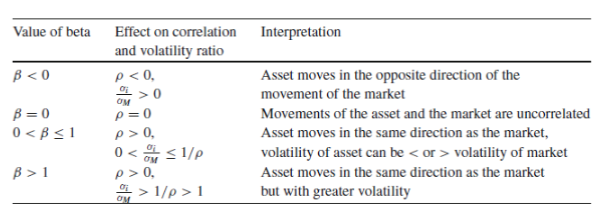
\includegraphics[width=1\textwidth]{images/beta.png}
    \caption{Beta}
\end{figure}
\FloatBarrier
\paragraph{Diversi vincoli per la portfolio optimization}
\begin{itemize}
    \item \textbf{Limiti superiori e inferiori per gli holders}: per regolare le proporzioni tra gli asset oppure obbligare l'investitore ad avere solo long positions ($w_i \geq 0$)
    \item \textbf{Limiti di turnover nell'acquisto/vendita}: Per stabilire un limite superiore alla proporzione della variazione degli holding da un periodo all'altro
    \item \textbf{Limiti di trading}: Per stabilire un limite inferiore alla produzione della variazione degli holding da un periodo all'altro
    \item \textbf{Dimensioni del portfolio}: Limiti sul numero di asset di un portfolio
\end{itemize}
\section{Portfolio Selection}
Quando un portfolio devia dall'expected return dell'investitore le sue posizioni devono essere riviste ribilanciando i pesi.\\[12pt]
Consideriamo un investitore con $m$ long securities con un orizzonte temporale, senza costi di transazione e investimento fisso iniziale
\begin{itemize}
    \item Il \textbf{tempo} tra presente e orizzonte viene \textbf{diviso} in $n$ periodi dove $t=0$ è l'inizio e $t=n$ è la fine
    \item \textbf{Alla fine} di ogni \textbf{periodo} $[t-1, \ t]$ la \textbf{proporzione} di \textbf{peso} investita in ogni posizione \textbf{viene rivista}
\end{itemize}
Il \textbf{cambiamento del market price} per un dato periodo è rappresentato dal \textbf{vettore di mercato}
$$x_t=(x_{t1},x_{t2},\dots,x_{tm})$$
Dove:
$$x_{ti}={{P_i(t)}\over{P_i(t-1)}}$$
Ovvero il \textit{rapporto tra close e opening price dell'i-esima security nel periodo}  $[t-1, \ t]$
La \textbf{distribuzione di pesi} tra le $m$ securities per un dato periodo $t$ è rappresentata dal \textbf{vettore di portfolio}
$$w_t=(w_{t1},w_{t2},\dots,w_{tm})$$
$$w\in W \ dove \ W=\{w\in \Re_+^m, \sum_{j=1}^m w_j=1\}$$
Quindi \textbf{un investimento} per \textbf{portfolio} $w_t$ produce un \textbf{incremento di peso} rispetto al vettore di mercato $x_t$ nel periodo $[t-1, \ t]$ di un fattore
$$w_t'\cdot x_t=\sum_{i=1}^mw_{tj}\cdot x_{tj}$$
Una \textbf{sequenza di investimenti} per una \textbf{selezione di} $n$ \textbf{vettori portfolio} $w_n=(w_1,w_2,\dots,w_n)$ risulta in un incremento di wealth di
$$S_n(w^n,x^n)=\prod_{t=1}^nw_t'\cdot x_t=\prod_{t=1}^n\sum_{j=1}^mw_{tj}w_{tj}$$
Con
\begin{itemize}
    \item $x^n=(x_1,\dots,x_n)$ sequenza di vettori prezzo corrispondenti agli $n$ periodi
    \item $S_n(w^n,x^n)$ è il fattore wealth ottenuto da $w^n$ rispetto alla sequenza di vettori mercato $x^n$
\end{itemize}
\paragraph{Definizione} Una strategia di portfolio selection per $n$ periodi di trading è una sequenza di $n$ scelte di vettori portfolio $w^n=(w_1,\dots,w_n)$ dove ogni $w_t\in W$.
\\Un algoritmo di portfolio selection è un algoritmo che produce una strategia di portfolio selection
$$S_n(w^n,x^n)\rightarrow S_n(ALG, x^n)$$
Per valutare le performance di questi algoritmi:
\begin{itemize}
    \item Confronto dei wealth factor
    \item Confronto dell'exponential growth rate
\end{itemize}
\subsection{Strategia Buy And Hold}
\begin{itemize}
    \item Allocare tutto il wealth lungo le $m$ security secondo $w_1\in W$
    \item Non eseguire trading
\end{itemize}
$$S_n(w_1,x^n)=\prod_{t=1}^n\sum_{j=1}^mw_{1j}x_{tj} $$
\subsection{Strategia Constant Rebalanced Portfolio (CRP)}
\begin{itemize}
    \item Strategia timing
    \item Utilizza la stessa distribuzione dei pesi in ogni periodo
    \item $CRP_w$ strategia con pesi fissi $w=(w_1,w_2,\dots,w_m)$
\end{itemize}
$$S_n(CRP_w, X^n)=\prod_{t=1}^n\sum_{j=1}^mw_jx_{tj}$$
\begin{itemize}
    \item Ribilanciamento dei pesi alla fine di ogni periodo, ovvero trovare $w^*$ tale che $max \ S_n(CRP_w,x^n)$
\end{itemize}
$CRP_{w^*}$ è migliore delle altre straategie di portfolio selection, ma irrealizzabile perché basata su previsioni del futuro di $x^n$
\end{document}